%% Models
%%=========================================

\chapter{Models}
\label{ch:models}
In this chapter we present the three models we created during our iterative development process. We present the {\tt VecRep} model in Section \ref{sec:repeat_vector}, and our two encoder-decoder based models {\tt EncDecReg} and {\tt EncDecAtt} are presented in Sections \ref{sec:regular_encoder_decoder} and \ref{sec:attention_encoder_decoder}.

%%=========================================

\section{Repeat Vector}
\label{sec:repeat_vector}
The first model, called {\tt VecRep} for short, has a similar structure to that of the encoder-decoder framework. The model consists of two groups of LSTMs. The first group reads the entire input and outputs its final hidden state. This hidden state is then repeated in the dimension of time, and inputted into a new group of LSTMs.

\begin{figure}[ht]
    \centering
    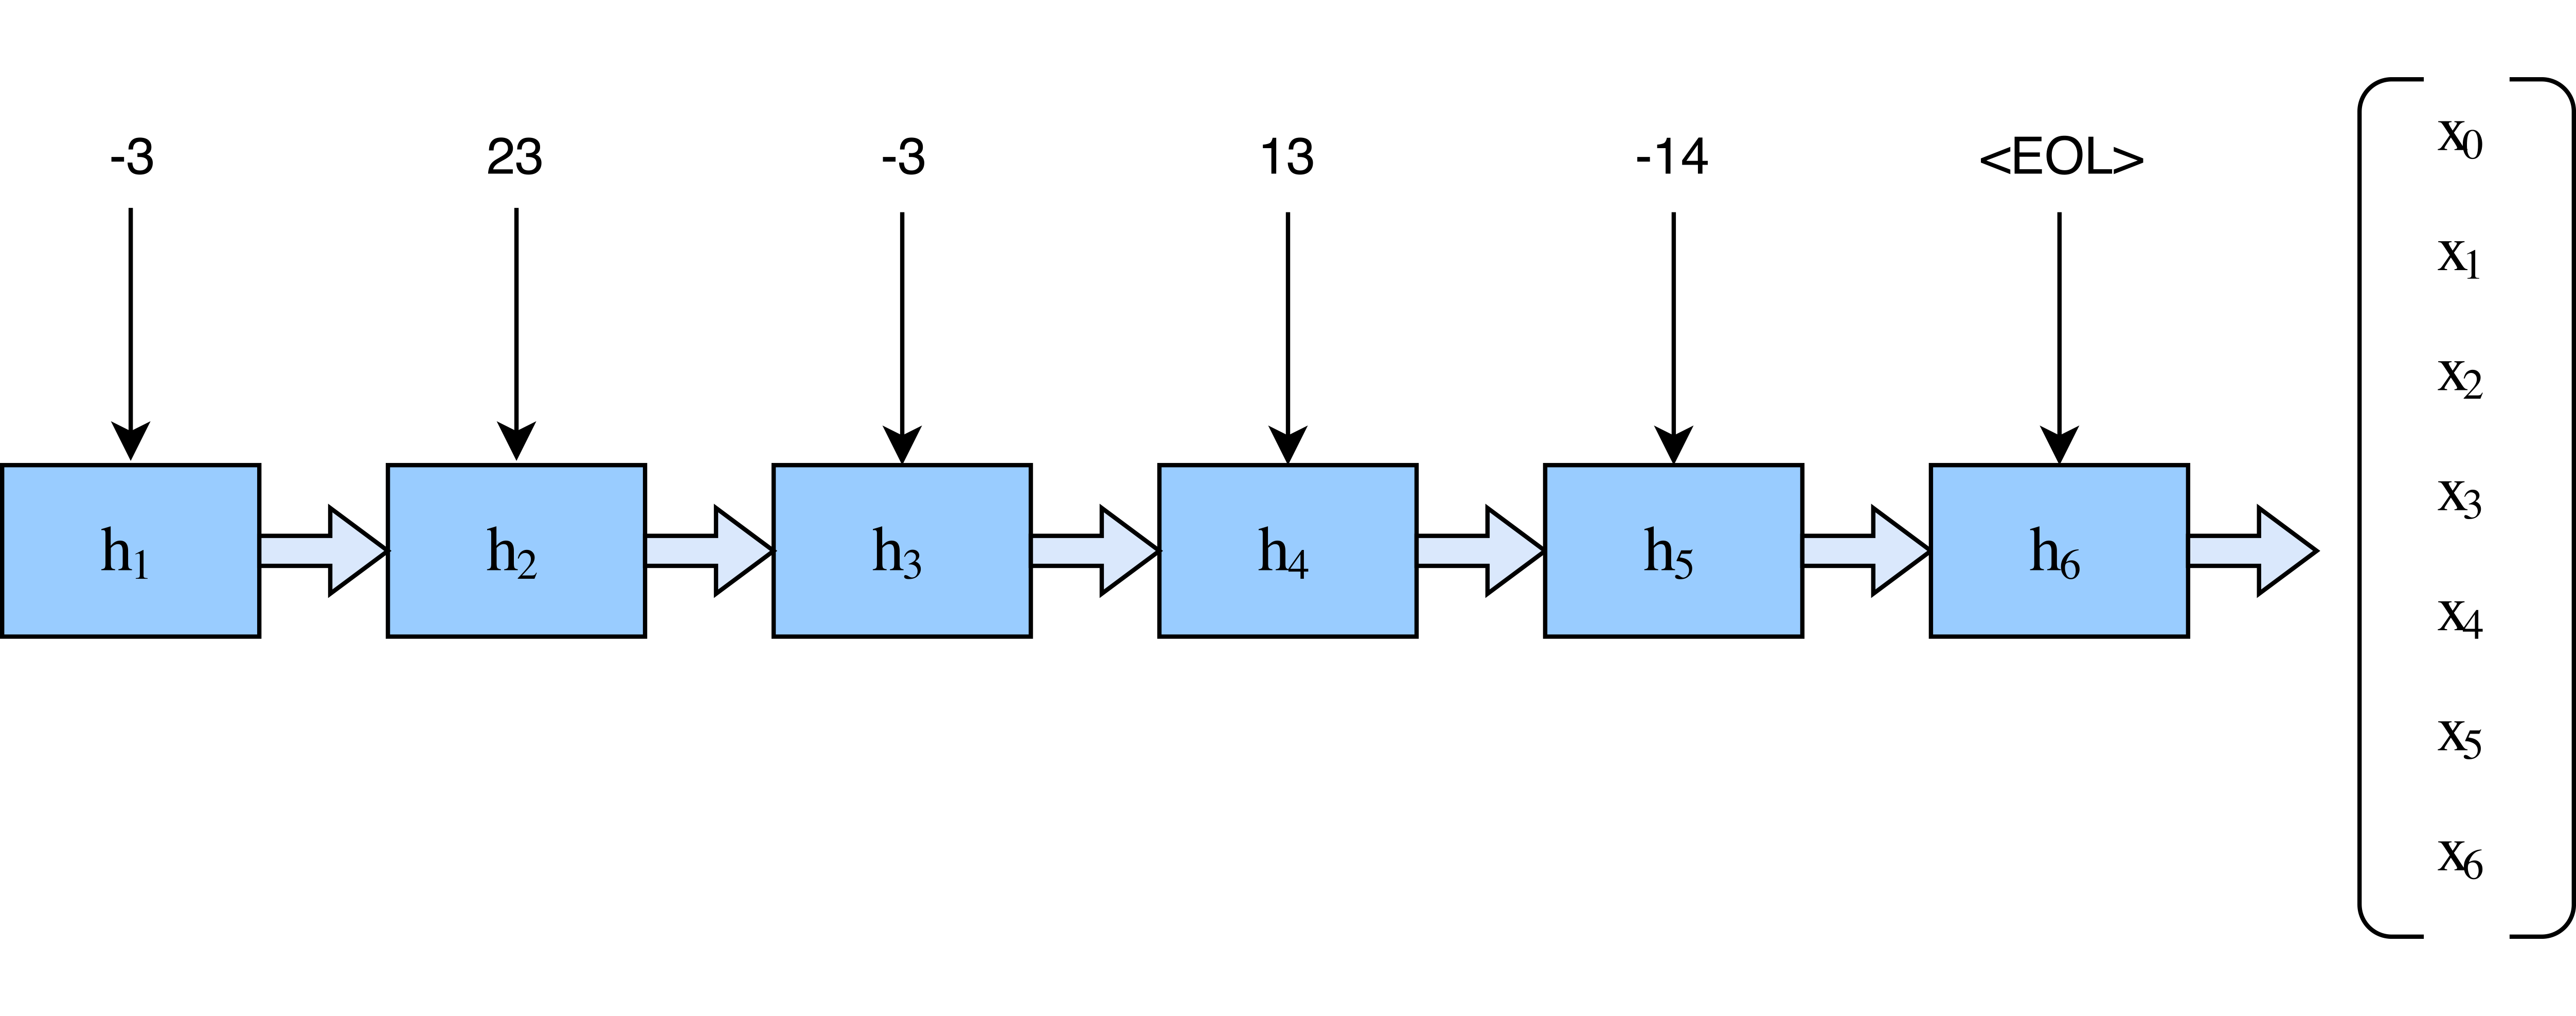
\includegraphics[width=0.7\textwidth]{fig/development_process/lstm-vector-projection-encoder.png}
    \caption{A LSTM outputting its final hidden state after reading a sequence}
    \label{fig:lstm-vector-projection-encoder}
\end{figure}

Figure \ref{fig:lstm-vector-projection-encoder} illustrates a regular LSTM that reads an input sequence and output its final hidden state. The output vector has a length equal to the number of units in the LSTM. As illustrated in Figure \ref{fig:lstm-vector-projection-decoder}, the hidden state from the LSTM is repeated \(N\) times, where \(N\) is the length of the output sequence. This means we take an output shape of {\tt (batch\_size, units)} from the first group of LSTMs, and turn it into a shape of {\tt (batch\_size, N, units)}.

\begin{figure}[ht]
    \centering
    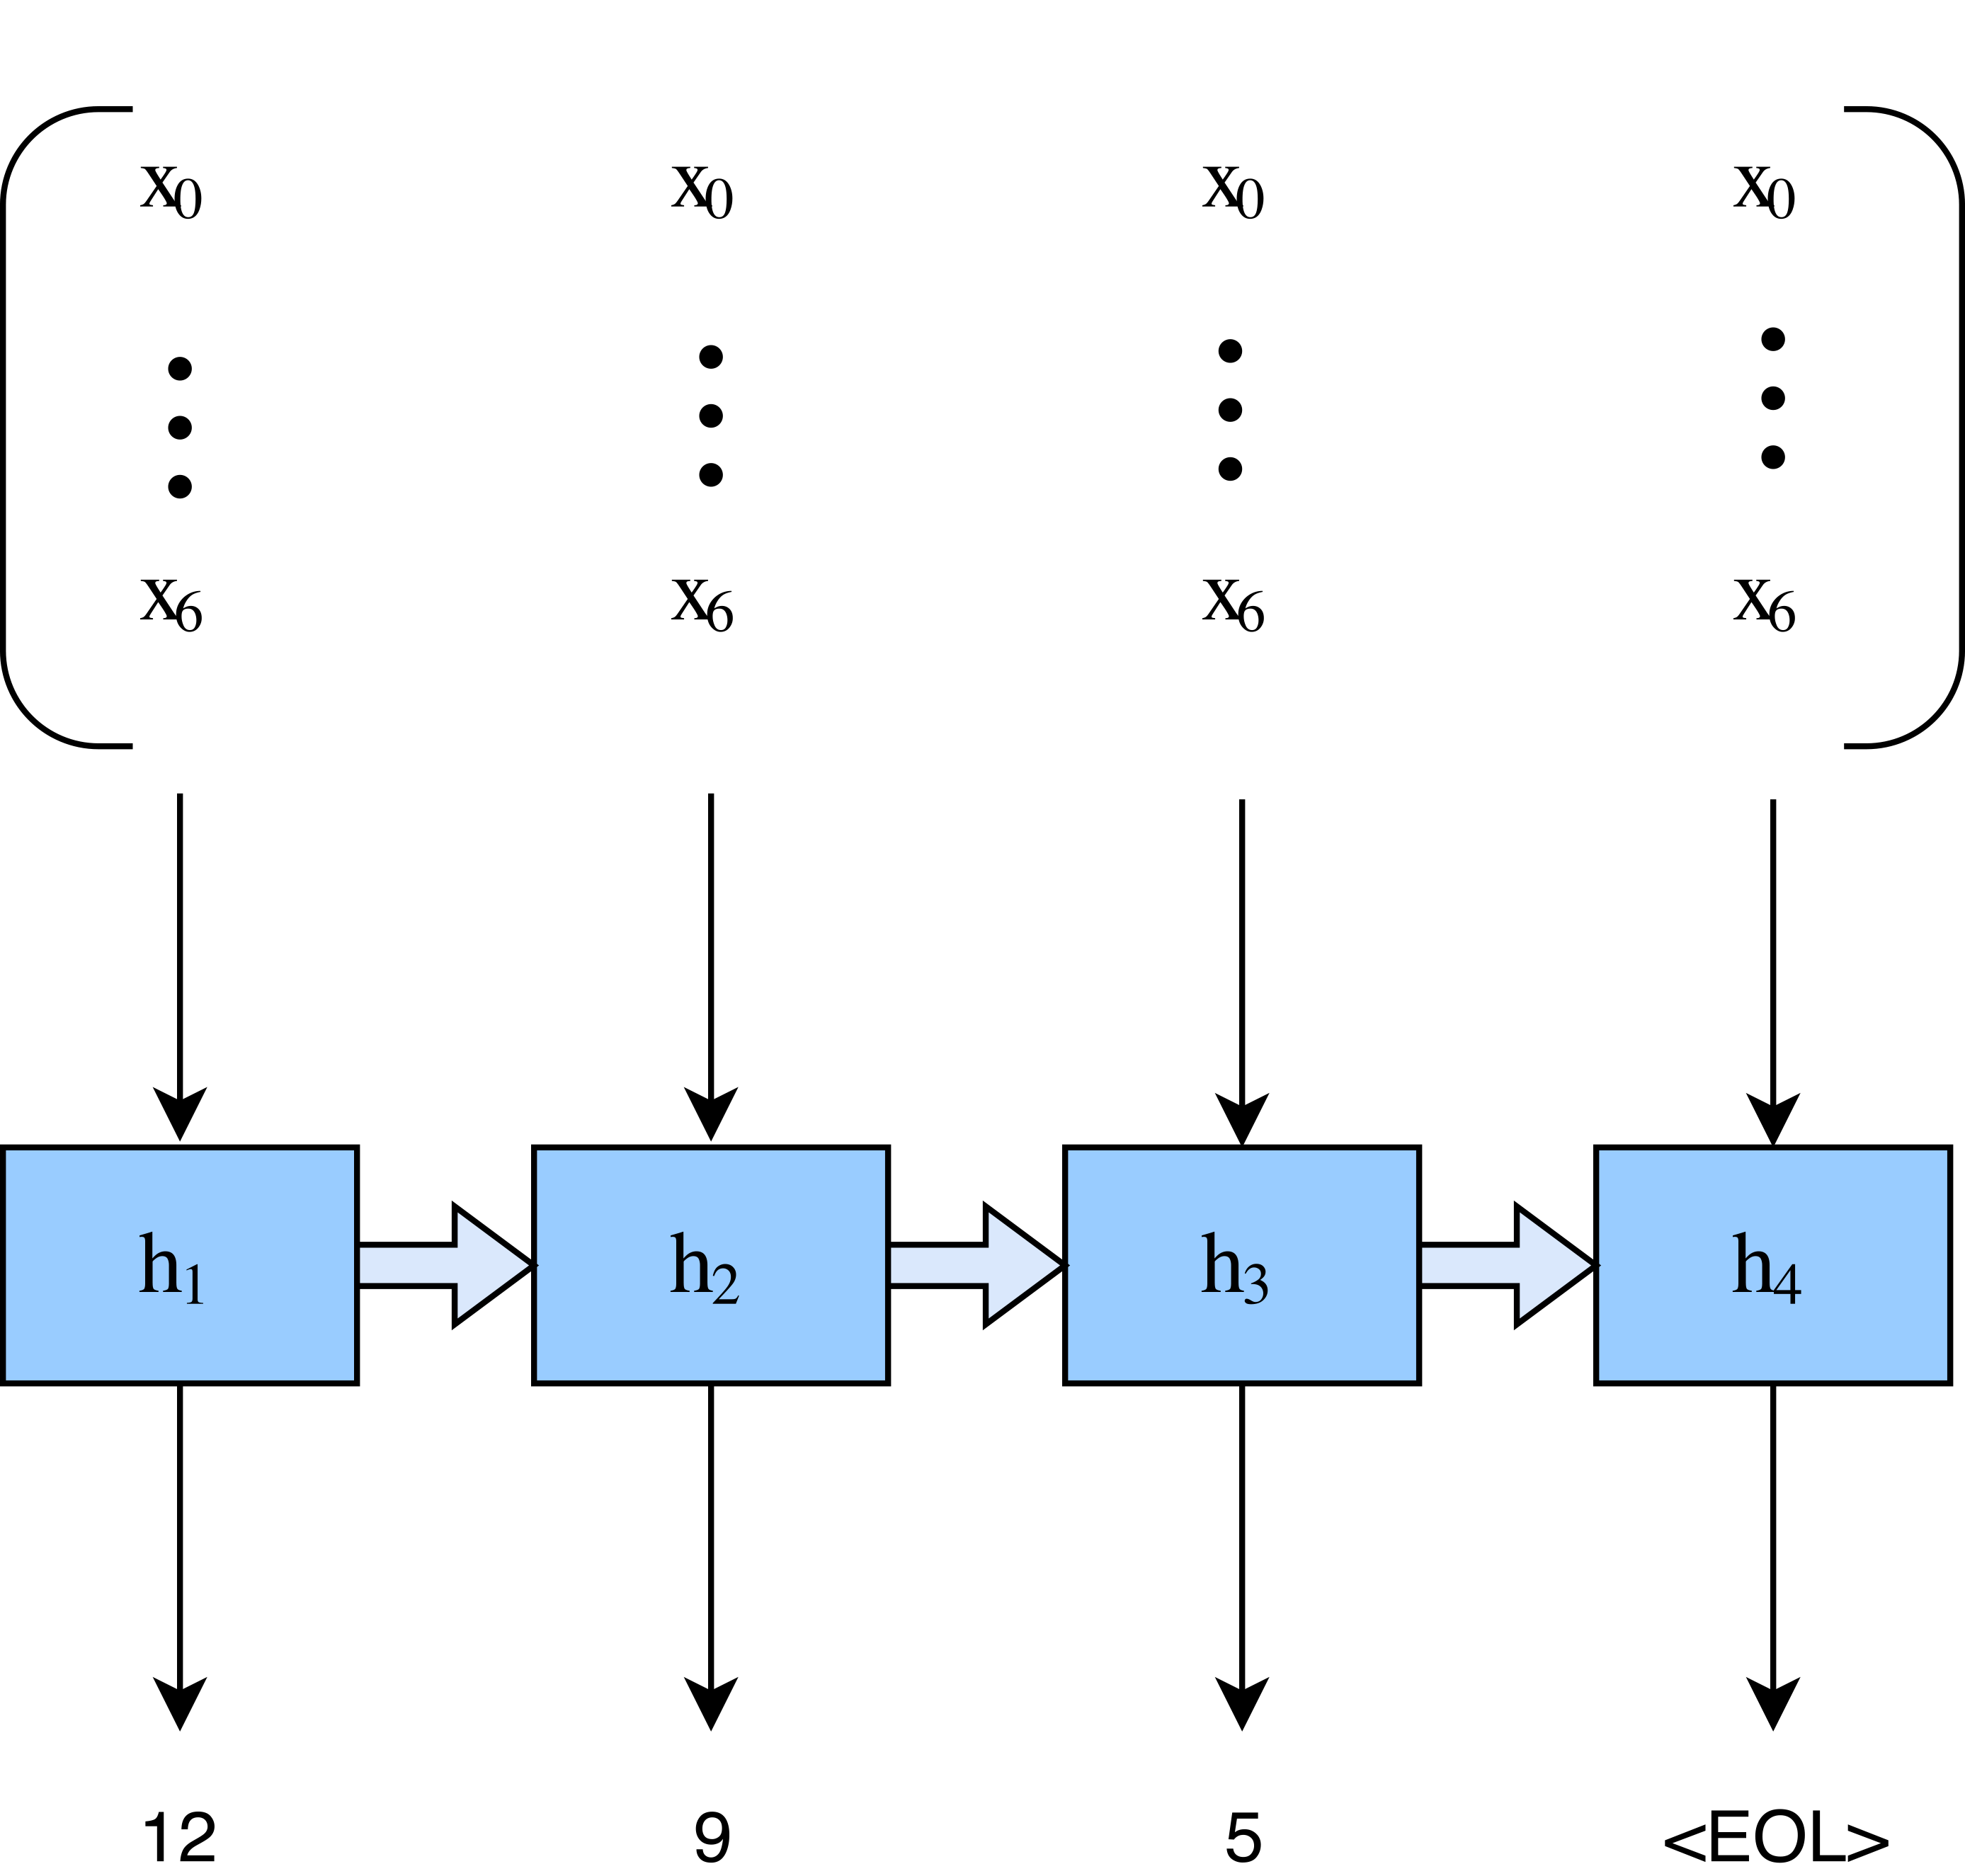
\includegraphics[width=0.5\textwidth]{fig/development_process/lstm-vector-projection-decoder.png}
    \caption{Repeating the output from a LSTM and feeding it to another LSTM}
    \label{fig:lstm-vector-projection-decoder}
\end{figure}

In this example, out output has a length of three characters, plus a special ``end of line" character. The resulting matrix of the repeated vector is then fed to another LSTM that reads each time step and output its hidden state for each iteration.

%%=========================================

\section{Regular Encoder-Decoder}
\label{sec:regular_encoder_decoder}
The second model implements the encoder-decoder framework. It is called {\tt EncDecReg} as it is the ``regular" encoder-decoder, unlike the last model. This model has certain similarities to the {\tt VecRep} model; also this one consists of two groups of LSTMs, where the first group encodes the input and the last group decodes.

However, in this model, we use the last hidden state of the encoder, instead of the output as with the {\tt VecRep} model. In addition, during testing and validation, the decoder feed its output back in as input. During training, instead of relying on the models own output, we use the actual labels. This is similar to the approach taken by \citep{bengio2015scheduled}.

This model also uses two embeddings, one for the input and one for the output. The input is embedded before the encoder reads the input, and the output embedding is applied on the fly when the decoder is reusing its own output as input. This is in contrast to the {\tt VecRep} model which only used embedding for the input data. Both the embeddings in this model is fully trainable.

%%=========================================

\section{Attention Encoder-Decoder}
\label{sec:attention_encoder_decoder}
The last model also implements the encoder-decoder framework, similarly to the {\tt EncDecReg} model. In addition, this model also implements the attention mechanism, and is named {\tt EncDecAtt} for short.

As explained in Section \ref{sec:attention_mechanism}, the attention mechanism allows the decoder to peek into the input. This is done by providing an additional list of states from the input. This is done by the decoder, by using the attention mechanism over the encoder LSTM states. The implementation of the attention mechanism used in this model is based on \citep{vinyals2015grammar}.

